\section{Simulation Evaluation} \label{sec:simulation}

We have developed a simulation framework for comparing schedules generated from \textsc{STAM} and \textsc{STFU} task lists to schedules generated from non-smoothed task lists.  Our simulation includes a stochastic energy harvesting process, a random task list and \textsc{STAM}/\textsc{STFU} task list generator, the scheduling processes, and an execution process.  We execute $n$ simulations on one task list per run, and generate task lists for $r$ runs.  Each task list consists of $k$ tasks.

\subsection{Task Generation}
The tasks are generated with random periods, durations, and energy requirements.  The periods and durations are distributed uniformly in discrete time steps measured in days, ranging respectively from 10 to 40 and from 1 to 4.  The energy is half-normally distributed, and proportional to the task's period (\emph{i.e.} a task requiring high energy is expected to run at a low frequency).

A random task list and its corresponding virtual task list generated by \textsc{STAM} and \textsc{STFU} are generated reiteratively until both lists are temporally schedulable.  We consider a task list temporally schedulable when its CPU utilization $U$ (from equation \ref{eqn:utilization} is less than 100\%.  We assume that the physical task list has less than 50% utilization, to better demonstrate our work.

\subsection{Energy Harvesting Model}
We use a simple model of a photovoltaic energy harvester, which converts solar irradiance $G$ into a current $I_c$, as a stochastic energy source for our simulation.  The energy withdrawn from the environment is modeled as a 3-state Markov chain (\cite{poggi2000stochastic,moser2007real}) representing three weather conditions (figure~\ref{fig:markov}).  At each discrete time step during the simulation the Markov chain is updated, and the energy generated added to an energy pool (\emph{i.e.} a battery).
\begin{figure}[htb]
\begin{center}
\label{fig:markov}
\caption{Markov Chain Weather Model.}
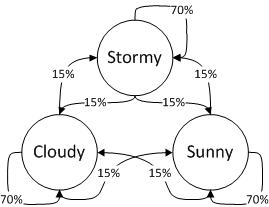
\includegraphics[scale=0.8]{markov.png}
\end{center}
\end{figure}
We generated a table of energy inputs to the system using the solar cell model that comes with Simulink's SimElectronics toolkit, configured with values from \cite{gonzalez2006model}.  
\begin{table}[h]
\begin{center}
\begin{tabular}{| l | l || l | l |}
\hline
\textbf{$G$ ($\frac{W}{m^2}$)} & \textbf{$I_c$ ($A$)} & \textbf{$G$ ($\frac{W}{m^2}$)} & \textbf{$I_c$ ($A$)} \\
\hline
50 & 0.190 & 175 & 0.665 \\
75 & 0.285 & 200 & 0.760 \\
100 & 0.380 & 225 & 0.855 \\
125 & 0.475 & 250 & 0.950 \\
150 & 0.570 & 275 & 1.045 \\
\hline
\end{tabular}
\end{center}
\label{tab:radiance}
\caption{Solar panel energy output}
\end{table}
The solar cell's current output with a battery load is related to its radiation input by the linear function $I_c = 0.0038G$.  We use the values of $G = 50, 100, 200 \frac{W}{m^2}$ to represent the stormy, cloudy, and sunny weather conditions in our weather model.

The output current of the photovoltaic cell, $I_c$, is governed by a two-diode formula given in \cite{marwali1997probabilistic} and modeled by the Simulink model.  The current flows into a battery, for which we use a linear model without relaxation effect.  The battery capacity at time $t$, $B_t$ is calculated using equation~\ref{eqn:batterycharge} per \cite{niyato2007sleep}.
\begin{equation}
 B_t = B_{t-1} + I_c \Delta t - I_d \Delta t
\label{eqn:batterycharge}
\end{equation}
where 
\begin{description}
\item[$B_{t-1}$] is the previous battery capacity
\item[$I_c$] is the charge current due to solar harvesting during $\Delta t$
\item[$I_d$] is the discharge current due to task execution during $\Delta t$
\end{description}
We represent $I_c$ and $I_d$  as constant averages during the interval $\Delta t$. Furthermore, the battery is
limited in capacity, such that if $B_t = B_{max}$ then any excess energy that is harvested is lost.

\subsection{Simulation Results}
We performed 1000 runs, with one run consisting of 100 simulations each on several task schedules using common random numbers (\emph{i.e.} using the same weather patterns).  Each simulation covered a 100-minute period, and if the battery charge dropped to 0 during the simulation we incremented a violation counter.  We recorded the number of violations produced during each run.  Figure \ref{fig:violationhist} shows a histogram of violations that occurred during a simulation with our chosen parameters.
\begin{figure}[htb]
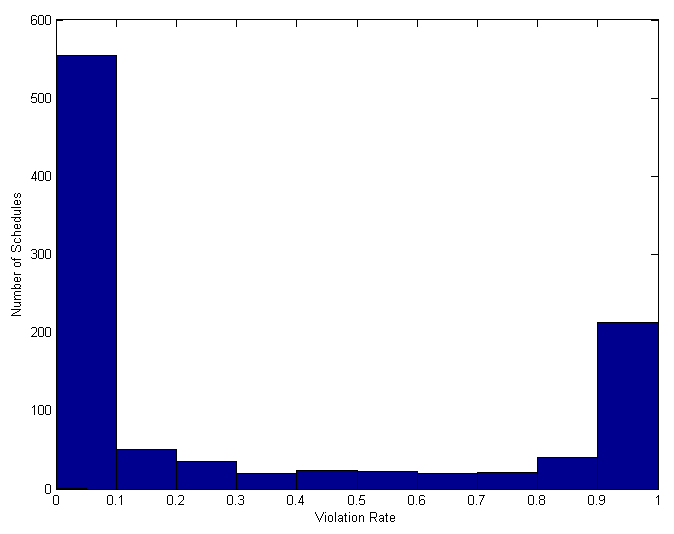
\includegraphics[scale=0.5]{violationhistogram.png}
\label{fig:violationhist}
\caption{Histogram of violation counts over 1000 runs.}
\end{figure}
Most of the random task lists were easy to schedule without energy violations, thanks to the 50\% duty cycle requirement we imposed on the physical task list.  Without restrictions beyond that of temporal schedulability, approximately 20% of runs had a 100% violation rate, indicating that it is realistic to require a low utilization on the physical task list.

We used earliest-deadline-first (\textsc{EDF}) and as-late-as-possible (\textsc{ALAP}) scheduling to schedule real tasks, \textsc{STAM} virtual tasks, and \textsc{STFU} virtual tasks.  In \textsc{EDF}, each task is scheduled as early as possible, in order of increasing deadline.  In \textsc{ALAP}, tasks are scheduled at the latest time possible such that no task misses its deadline.  \textsc{ALAP} is an energy-ignorant version of LSA, which means that it can be scheduled statically without a sophisticated energy prediction model.
\begin{table}[h]
\begin{center}
\begin{tabular}{| l | l |}
\hline
\textbf{Algorithm} & \textbf{Violations} \\
\hline
EDF & 5.3 \\
EDF \textsc{STAM} & 4.6 \\
EDF \textsc{STFU} & 2.4 \\
ALAP & 2.1 \\
ALAP \textsc{STAM} & 1.8 \\
\hline
\end{tabular}
\end{center}
\label{tab:simresults}
\caption{Violations per 100 simulations}
\end{table}
Table~\ref{tab:simresults} shows the simulation results for the scheduling algorithms we tested.  As expected, \textsc{EDF}---the optimal periodic scheduling algorithm in systems with unlimited energy---resulted in the most violations.  Schedules generated by applying the \textsc{EDF} scheduler to the virtual task lists generated by the \textsc{STAM} and \textsc{STFU} algorithms performed better: \textsc{STAM} resulted in about 0.7 fewer violations per 100 simulations, and \textsc{STFU} resulted in about 2.9 fewer violations per 100 simulations.

The \textsc{ALAP} algorithm resulted in 3.2 fewer violations per 100 simulations than \textsc{EDF}, and when run on \textsc{STAM} virtual tasks \textsc{ALAP} resulted in 3.5 fewer violations.  Task lists with high utilization are difficult to schedule with \textsc{ALAP}, so we did not schedule \textsc{STFU} virtual tasks with \textsc{ALAP}; however, scheduling \textsc{STFU} tasks with EDF produces results close to those of \textsc{ALAP}-based methods.





































